\section{课程名称}

数据库新技术。

\section{实验项目名称}

分布式数据库系统。

\section{实验原理}

本章将介绍本次分布式数据库系统实验涉及到的相关技术的实验原理,包括SQL词法解析技术和RPC远程函数调用技术。

\subsection{SQL词法解析}

SQL的词法解析可以分为如下步骤:
\begin{enumerate}
    \item 词法分析。将SQL字符串拆分成包含关键词识别的字符段(Tokens)。
    \item 语法分析。利用自顶向下或自底向上的算法,将tokens解析为语法树。
    \item 错误检测。对语法树进行错误检测、恢复和提示。
\end{enumerate}

本实验着重实现了词法分析和语法分析的阶段,其流程如图\ref{fig:sql-parse}所示,其具体实现将在后续章节中详细介绍。

\begin{figure}[H]
    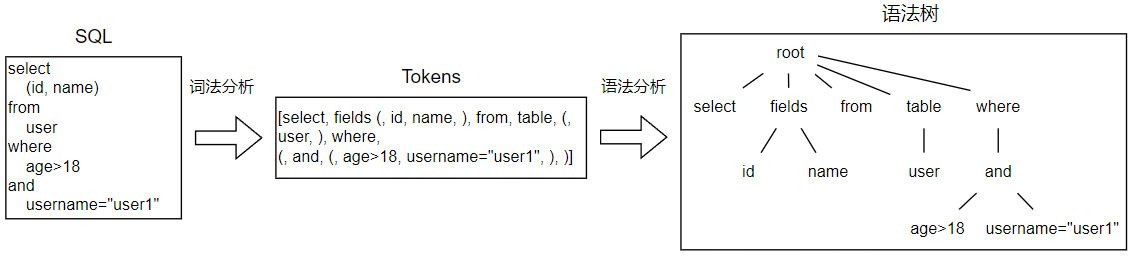
\includegraphics[width=\textwidth]{examples/sql解析流程.png}
    \centering
    \caption{SQL解析流程}
    \label{fig:sql-parse}
\end{figure}

在词法分析阶段,会找出SQL字符串中的关键词,包括关键字、操作符、开闭合标志、占位符、空格、文本、数字等,并进行分词,将关键词分割为若干token。

在语法分析阶段,会将token序列转换为语法树,这一步骤比较多样,不同的解析器可能具有不同的结果,本实验也是尝试独立编写了一个简单的解析器。

\subsection{RPC远程函数调用}

RPC是一种远程过程调用协议,它是一种通过网络从远程计算机程序上请求服务,而不需要了解底层网络技术的协议。一个完整的RPC架构里面包含了四个核心的组件,分别是客户端、客户端存根、服务端、服务端存根。

\begin{figure}[H]
    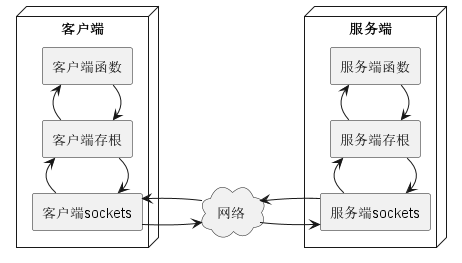
\includegraphics[width=0.7\textwidth]{examples/rpc原理.png}
    \centering
    \caption{RPC原理}
    \label{fig:rpc}
\end{figure}

如图\ref{fig:rpc}所示,当客户端请求RPC服务时,会通过存根打包请求参数,然后通过网络发送给服务端;服务端存根接收请求,将消息解包后调用本地方法,并将结果返回到客户端。为了使得请求可以在网络中传递,往往需要对数据进行序列化操作。

\section{实验目的}

实现一款简易的分布式数据库系统,能够支持基本的数据库操作,提升自己对数据库系统的理解和工程能力。

\section{实验内容}

设计和开发小型分布式图书馆系统的数据库系统,要求如下:
\begin{enumerate}
    \item 数据必须存放在至少3个站点上,数据的划分对用户完全透明。
    \item 系统必须支持基本的SQL查询语句(可以不包含嵌套),并能将查询结果反映到界面上。
    \item 系统必须支持数据划分,可以选择支持水平划分,垂直划分,水平十垂直划分或者混合划分。
    \item 用户查询要进行分解和优化,然后转交底层数据库管理系统执行。
    \item 各分站点服务器界面上必须能显示出所接受和发送的命令,以及命令的处理过程。必须直接显示到界面上,不允许记录到log文件中。
    \item 主站点要显示生成查询分解和优化过程。
\end{enumerate}

\section{实验环境}

开发环境:
\begin{itemize}
    \item Visual Studio Code 1.82.2。用于进行代码编写的工具。
    \item Miniconda 4.12.0。Python环境的管理工具。
    \item Python 3.8.16。本实验所使用的开发语言。
\end{itemize}

依赖:
\begin{itemize}
    \item Anytree 2.11.1。搭建树结构的工具包,支持节点创建和树的遍历操作。
    \item Pandas 1.5.3。数据处理工具包,可以读写本地文件,并以数据表的形式组织、查看和修改。
    \item Rpyc 5.3.1。用于RPC操作的工具包。
\end{itemize}